\documentclass[12pt, a4paper]{book}

\usepackage{fancyhdr}
\usepackage[left=4cm, right=4cm, top=4cm, bottom=4cm]{geometry}
\usepackage[utf8]{inputenc}
\usepackage[table]{xcolor}
\usepackage{hyperref}
\usepackage{amsmath}
\usepackage{enumitem}
\usepackage{graphicx}
\usepackage{amsfonts}
\usepackage{color,soul}
\usepackage{booktabs}
\usepackage{subcaption}
\usepackage[justification=centering]{caption}
\usepackage{xepersian}

\DeclareMathOperator*{\argmax}{argmax}
\DeclareMathOperator*{\argmin}{argmin}
\newcolumntype{L}{>{$}l<{$}} % math-mode version of "l" column type

\newcommand{\coursetitle}{بازیابی اطلاعات}
\newcommand{\doctitle}{تمرین دوم}
\newcommand{\name}{محمدرضا غفرانی}
\newcommand{\studentno}{400131076}
\newcommand{\todaydate}{\today}

\settextfont{XB Kayhan}

\pagestyle{fancy}
\lhead{\textbf{\doctitle}}
\rhead{\name}

\begin{document}

\begin{flushleft}
    \name \\
    \studentno \\
    \todaydate
\end{flushleft}

\begin{center}
    \huge
    \textbf{\coursetitle}
    \break
    \large
    \doctitle
\end{center}

% suppress the fancy header on the first page only
\thispagestyle{plain}

\section*{بخش دوم}

در این قسمت ما از مدل \lr{roberta-base} برای به دست آوردن بازنمایی برداری جملات استفاده کردیم.
ساختار این مدل بسیار شبیه به مدل \lr{BERT} است اما با تغییراتی که در آموزش مدل داشته‌اند توانسته‌اند
به نتایج بهتری در وظایف گوناگون دست یابند.

این مدل را ما با استفاده از کتابخانه \lr{HuggingFace} بارگیری و استفاده کرده‌ایم.
از آن جا که این مدل \lr{tokenizer} خاص خود را دارد، بنابراین از همان برای تبدیل کلمات به
توکن‌ها و در ادامه برای تبدیل توکن‌ها به شناسه استفاده کرده‌ایم.

برای تبدیل جملات به بردار‌، از میانگین‌گیری بازنمایی که آخرین لایه مخفی مدل به ازای
هر کلمه وجود دارد استفاده کرده‌ایم. برای آن که سرعت اجرای کد بیشتر شود، علاوه بر بهره‌گیری از
\lr{GPU}، از تکنیک \lr{batching} و ذخیره بردار‌های متناظر مجموعه داده آموزشی برای جلوگیری از
محاسبه مجدد آن‌ها استفاده کرده‌ایم.

\section*{بخش سوم}

ما برای طراحی شبکه \lr{siamese} از پیشنهاد‌های موجود در صورت سوال استفاده کرده‌ و آزمایش‌های مختلفی را برای
به دست آوردن بهترین ترکیب آن انجام داده‌ایم. \autoref{siamese} شمای کلی شبکه \lr{siamese} طراحی شده را نشان می‌دهد.
در ادامه جزئیات مربوط به هر کدام از بخش‌های مختلف آن را بررسی می‌کنیم.

\begin{figure}[h]
    \centering
    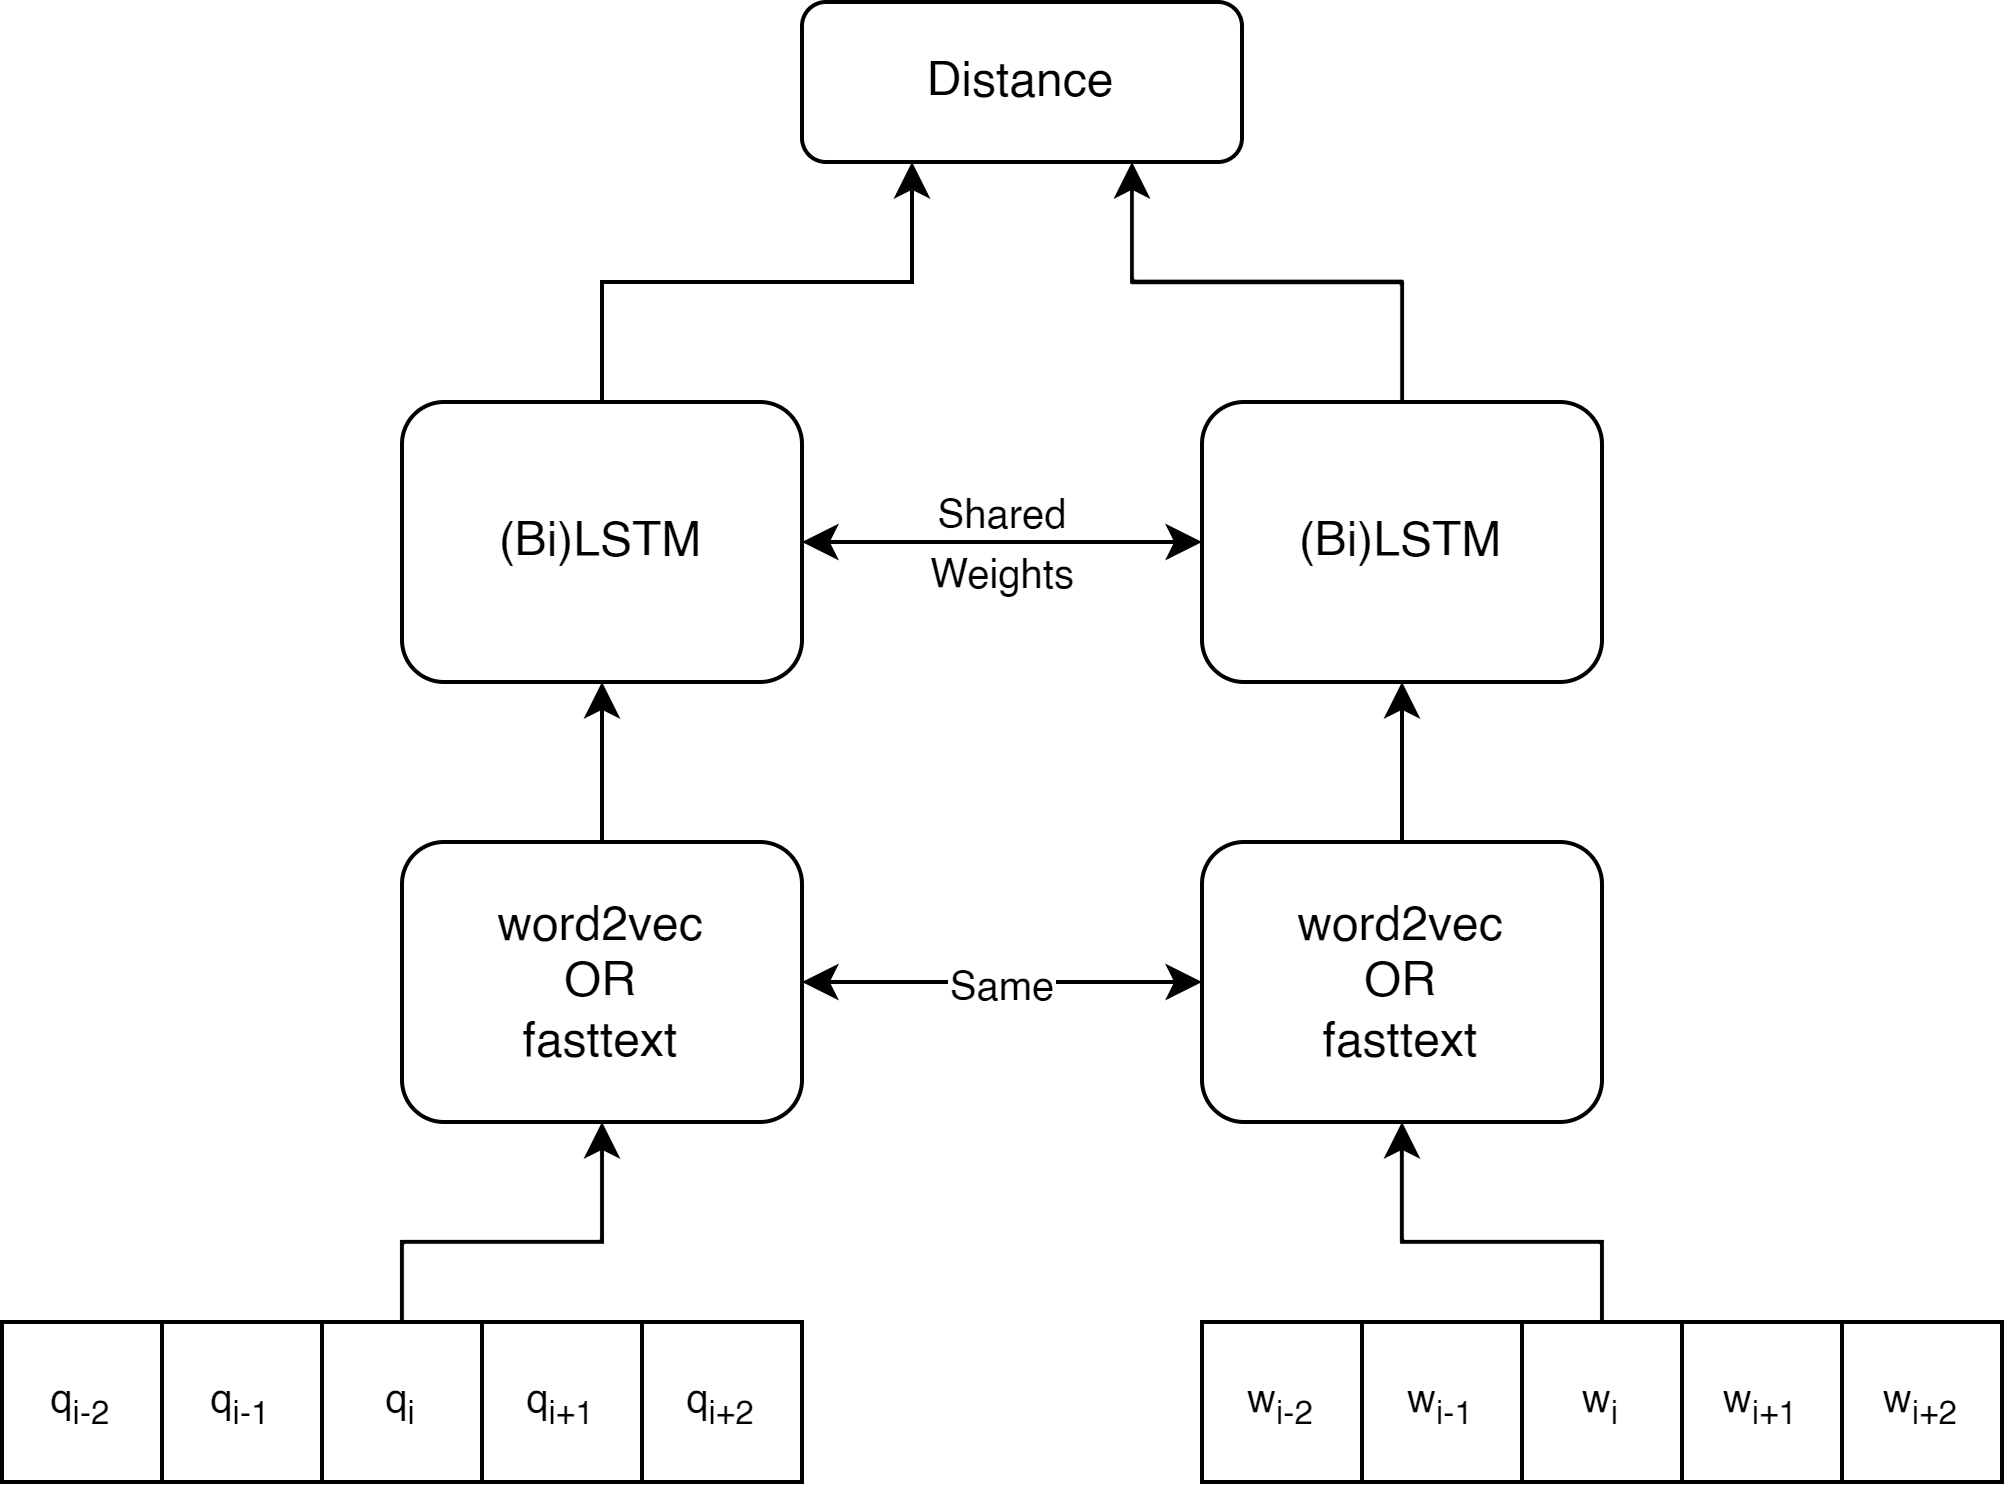
\includegraphics[width=0.8\linewidth]{images/siamese.png}
    \caption{شمای کلی شبکه \lr{siamese}}
    \label{siamese}
\end{figure}

\begin{itemize}
    \item \textbf{بازنمایی ورودی شبکه.} ما از هر دو بازنمایی \lr{fasttext} و \lr{word2vec} برای
    بازنمایی کلمات ورودی به لایه \lr{LSTM} استفاده کرده‌ایم. این بازنمایی‌ها در حین آموزش شبکه اصطلاحا
    \lr{freeze} شده بودند و تغییر نمی‌کردند.
     ما از مدل ازپیش‌آموزش‌دیده \lr{word2vec-google-news-300}
    به عنوان مدل \lr{word2vec} و از \lr{fasttext-wiki-news-subwords-300} به عنوان مدل \lr{fasttext}
    استفاده کردیم. هر دو این مدل‌ها با استفاده از کتابخانه \lr{gensim} بارگیری شدند و هر کدام هر کلمه را به یک بردار
    ۳۰۰ بعدی نگاشت می‌کردند.
    \item \textbf{معماری شبکه \lr{LSTM} استفاده شده.} ما هر دو معماری یک‌جهته و دوجهته را برای مدل
    \lr{LSTM} بررسی و ارزیابی کردیم. در حالت تک‌جهته حالت مخفی آخرین شبکه \lr{LSTM} به عنوان بازنمایی جمله استفاده
    می‌شود و در حالت شبکه \lr{LSTM} دو جهته ادغام حالت‌های مخفی شبکه \lr{LSTM} به ازای توکن‌های اول و آخر
    به عنوان بردار بازنمایی جمله استفاده می‌شود.
    \item \textbf{فاصله استفاده شده برای اندازه‌گیری خروجی شبکه \lr{LSTM}.} ما برای بررسی شباهت دو بازنمایی
    تولید شده توسط شبکه \lr{LSTM} از فاصله کسینوسی و استفاده از یک شبکه خطی برای تعیین فاصله دو بردار استفاده
    کرده‌ایم. در حالت استفاده از فاصله کسینوسی هر چه فاصله دو بردار به یک نزدیک‌تر باشد دو بردار‌ را به
    هم شبیه‌تر می‌نامیم. در هنگام استفاده از شبکه خطی نیز دو بردار ورودی را با هم ترکیب کرده و به شبکه خطی
    می‌دهیم تا اگر دو بازنمایی معنای یکسانی داشتند خروجی یک و در غیر این صورت خروجی صفر بدهد.
\end{itemize}

\section*{بخش چهارم}

نتایج استفاده از شبکه \lr{RoBERTa} و شبکه \lr{siamese} در \autoref{results} آورده شده است.
همان‌طور که مشاهده می‌شود مدل \lr{RoBERTa} عملکرد بسیار بهتری نسبت به شبکه‌های \lr{siamese} طراحی شده دارد.
از طرف دیگر نکته جالبی که در شبکه‌های \lr{siamese} دیده می‌شود، تاثیر فاصله کسینوسی در عملکرد بهتر مدل است.
در شبکه‌هایی که از این فاصله استفاده شده است به وضوح نتایج بهتر بوده است. با توجه به آن که این شبکه‌هایی
که از فاصله کسینوسی برای تعیین شباهت دو جمله استفاده کرده‌اند در زمان آموزش مدل دقت‌های بالایی ارائه نکرده‌اند،
بنابراین به نظر می‌رسد در این شبکه‌ها \lr{generalization} بهتر اتفاق باشد و شبکه \lr{LSTM} تلاش کرده بردار
خروجی را به نحوی بدهد که با یک مقایسه نسبتا ساده بتوان شبیه بودن یا نبودن متون را تشخیص داد.
نکته بعدی که مورد انتظار بود بهتر عملکرد شبکه \lr{LSTM} در گذر از یک جهته به دو‌جهته است.
گرچه بهترین عملکرد شبکه \lr{siamese} در زمان استفاده از \lr{LSTM} تک جهته اتفاق افتاده است اما
این روند را می‌توان به طور کلی مشاهده کرد.

\begin{table}[h]
    \centering
    \setLTR
    \caption{نتایج ارزیابی مدل‌های \lr{RoBERTa} و \lr{siamese} در بازیابی اطلاعات}
    \label{results}
    \begin{tabular}{c|c|c|c|c}
         مدل & \lr{MAP} & \lr{MRR} & \lr{AP@5} & \lr{AP@10} \\
         \hline
        \lr{RoBERTa} & $0.45$ & $0.76$ & $0.49$ & $0.34$ \\
        \lr{word2vec+LSTM+Linear} & $0.006$ & $0.005$ & $0.004$ & $0.002$ \\
        \lr{word2vec+LSTM+Cosine} & $0.26$ & $0.57$ & $0.29$ & $0.21$ \\
        \lr{word2vec+BiLSTM+Linear} & $7 \times 10^{-7}$ & $0.003$ & $0.001$ & $0.0006$ \\
        \lr{word2vec+BiLSTM+Cosine} & $0.21$ & $0.53$ & $0.26$ & $0.18$ \\
        \lr{fasttext+LSTM+Linear} & $0.0002$ & $0.003$ & $0.01$ & $0.002$ \\
        \lr{fasttext+LSTM+Cosine} & $0.18$ & $0.50$ & $0.22$ & $0.16$ \\
        \lr{fasttext+BiLSTM+Linear} & $0.0$ & $0.002$ & $0.0$ & $0.0$ \\
        \lr{fasttext+BiLSTM+Cosine} & $0.22$ & $0.55$ & $0.27$ & $0.19$ \\
    \end{tabular}
\end{table}


\end{document}